
\subsubsection{Odd Cyclic Extensions} \label{case_Cp}

For the first case, we assume that $d$ is odd. Following the observation in Remark \ref{rem_radical}, we will calculate $\Cp(\Theta_d)$ for each finite place $\pp$ of some subfield of $F^{C_{\rad(d)}}$. However, before we calculate these terms explicitly for distinct cases, we prove a technical result that considerably simplifies the calculations of $\Dp(\Theta_d)$.

\begin{lemma}
    Let $q$ be an odd prime and $L/K$ a Galois extension of number fields such that $\Gal(L/K)=C_q$, and let $\pp$ be a prime in $K$. Let $E/\QQ$ be an elliptic curve and $\Theta_q=C_1-C_q\in B(C_q)$. Then by changing the model of $E$ over $K$, and therefore by rescaling the discriminat of $E$, $\Dp(\Theta_q)$ does not change up to squares.
\end{lemma}
\begin{proof}
    Let $\Delta_E,\Delta_E'$ be the discrimiants of two models of $E$ over $K$, and let $\lambda=(\Delta_E'/\Delta_E)^{1/12}\in K$. Write $\Dp'(\Theta_q)$ and $\Dp(\Theta_q)$ for the value usual terms using $\Delta_E$ and $\Delta_E'$ as discriminants, respectively. Then a simple calculation shows that
    
    $$\Dp(\Theta_q)=\frac{\prod_{\fP\mid\fp}|\lambda|_\fP}{|\lambda|_\pp}\Dp'(\Theta_q).$$
    Hence, the result will follow by showing that $\prod_{\fP\mid\fp}|\lambda|_\fP/|\lambda|_\pp\in\QQss$. 
    
    There are three cases, depending on the splitting behaviour of $\pp$ in $F$. 
    \begin{itemize}
        \item If $\pp$ splits, then there are $q$ primes above $\pp$ with the same residue field and normalized valuation. Hence $\prod_{\fP\mid\fp}|\lambda|_\fP=|\lambda|_\pp^q$.
        \item If $\pp$ is inert, then there is one prime $\fP$ above $\pp$ whose residue field is a degree $q$ extension and with the same normalized valuation. Hence $|\lambda|_\fP=|\lambda|_\pp^q$.
        \item If $\pp$ ramifies, then there is one prime $\fP$ above $\pp$, with equal residue field but with normalized valuation satisfying $\nu_\fP(\lambda)=q\mu_\pp(\lambda)$. Hence $|\lambda|_\fP=|\lambda|_\pp^q$ too.
    \end{itemize}
    Hence, we always have that 
    $$\frac{\prod_{\fP\mid\fp}|\lambda|_\fP}{|\lambda|_\pp}=|\lambda|_\pp^{q-1}\in\QQss$$
\end{proof}

The great advantage of this result is that once a prime $\pp$ has been chosen in some subfield of $F^{C_{\rad(d)}}$, we will be able to assume that $\Delta_E=\Delta_{E,\pp}^{\min}$. 

To prove Theorem \ref{thm_consistent_cyclic} for odd $d$, we first calculate $\Cp(\Theta_d)$ for simple cases, and then we use them to prove the general case. The following lemmas build on this idea.

\begin{lemma}\label{lem_Cp}
    Let $q$ be an odd rational prime, $F/K$ a Galois extension of number fields such that $\Gal(F/K)=C_q$ and $E/\QQ$ an elliptic curve with semistable reduction at $2$ and $3$. If $\Theta_q=C_1-C_q$, then 
    $$C(\Theta_q)=\frac{C_{E/F}}{C_{E/K}}$$
    is a norm from $\QQ(\sqrt{q^*})$.
\end{lemma}

\begin{proof}
    Fix some prime $\pp$ in $K$, and assume that $\Delta_E=\Delta_{E,\pp}^{\min}$. We calculate $\Cp(\Theta_q)$ depending on the reduction type of $\pp$. Primes $\pp$ of good reduction yield no non-trivial factors since $\Tp(\Theta_q)=\Dp(\Theta_q)=1$. Hence, we may only consider from now on primes of bad reduction. We also note since the extension $L/K$ is cyclic, the splitting behaviour of $\pp$ in $L$ is determined by the ramification index $e_\pp$ and the residual degree $f_\pp$. 
    
    If $\pp$ has multiplicative reduction, then $D_{\fP\mid\pp}(\Theta_q)=1$ and Table \ref{table_Cp} records $T_{\fP\mid\pp}(\Theta_q)$ depending on $e_\pp$ and $f_\pp$, where and the entries for split and non-split multiplicative reduction of type $\mathrm{I}_n$ are separated by a ``;''. To complete these calculations, we use repeatedly Proposition \ref{prop_semi_red} and Lemmas \ref{lem_mult_tam} and \ref{lem_add_tam}. We also use Notation \ref{not_n}.

    \begin{table}[!ht]
        \centering
        \begin{tabular}{|l|l|l|l|l|}
        \hline
        $e_\pp$ & $f_\pp$  & $T_{\fP\mid \pp}(C_q)$ & $T_{\fP\mid \pp}(C_1)$  & $\Tp(\Theta_q)$ \\ \hline
        $1$ & $1$ & $n;\tilde{n}$ & $n^q;\tilde{n}^q$ & $\square$ \\ \hline
        $q$ & $1$ & $n;\tilde{n}$ & $qn;\tilde{n}$ & $q\square;\square$ \\ \hline
        $1$ & $q$ & $n;\tilde{n}$ & $n;\tilde{n}$ & $\square$ \\ \hline
        \end{tabular}
        \caption{Contribution of semistable reduction primes in a $C_q$ extension.}
        \label{table_Cp}
    \end{table}

    Since $q$ is indeed a norm from $\QQ(\sqrt{q^*})$ by Lemma \ref{p-norm}, it follows that $\Tp(\Theta_q)$ is a norm from $\QQ(\sqrt{q^*})$ as well.

    Now assume $\pp$ has additive reduction, and let $p\ZZ=\pp\cap\QQ$. By assumption, $p\neq2,3$. We note that $D_{\fP\mid\pp}(\Theta_q)=1$ unless $\pp$ ramifies in $F/K$, and in that case it is a power of $N_{K/\QQ}(\pp)=p^s$. If $s$ is even, then $D_{\fP\mid\pp}(\Theta_q)\in\QQss$, so assume instead that $s$ is odd. If $L_\fP/K_\pp$ is wildly ramified, then $p=q$ is a norm from $\QQ(\sqrt{q^*})$. If $L_\fP/K_\pp$ is tamely ramified, then by Proposition \ref{prop_totally_ramified}, it follows that $q\mid p^s-1$ and therefore 
    \begin{equation}
        \left(\frac{q^*}{p}\right)=\left(\frac{p}{q}\right)=\left(\frac{p^s}{q}\right)=1
    \end{equation}
    Therefore, $p$ splits in $\QQ(\sqrt{q^*})$ and by Corollary \ref{cor_psplit_pnorm}, it follows that $p$ is a norm from $\QQ(\sqrt{q^*})$. 
    
    Finally, we compute $\Tp(\Theta_q)$. Note that since $q$ is odd, any inertia degree is odd and therefore if $\fP$ is any prime in $F$ above $\pp$, $\sqrt{D}\in K_\pp$ if and only if $\sqrt{D}\in L_\fP$ for any $D\in\QQ$. Moreover, if $q\neq 3$, then $\gcd(e_{\fP\mid\pp},12)=1$ and by Lemma \ref{lem_add_tam}, $c_\pp(E/K)=c_\fP(E/F)$. This implies that $$\Tp(\Theta_q)=c_\pp(E/K)^{\#\{\fP\mid\pp\}-1}\in\QQss$$ since the number of primes $\fP$ in $L$ above $\fp$ is odd. If $q=3$ and $\pp$ is unramified in $L/K$, then $e_{\fP\mid\pp}=1$ and the same reasoning shows that $\Tp(\Theta_q)=1$. Hence, assume $L_\fP/K_\pp$ is ramified and let $n=\nu_\pp(\Delta_{E,\pp}^{\min})$ be the valuation of the minimal discriminant of $E$ at $\pp$. By Lemma \ref{lem_add_tam}, we can obtain factors of $2$ and $3$. Since $3$ is a norm from $\QQ(\sqrt{-3})$, we only need to take care of the factors of $2$, which can only arise if $F_\fP/K_\pp$ is ramified, $\gcd(n,12)=2$ and $\sqrt{\Delta}\not\in K_\pp$. However, Lemma \ref{lem_nottwo} shows that these conditions cannot arise, and therefore $\Tp(\Theta_q)$ is a norm from $\QQ(\sqrt{-3})$ as desired.
\end{proof}

Next, we prove an analogous result for $C_{qr}$ extensions, where $q$ and $r$ are distinct odd rational primes.

\begin{lemma}\label{lem_Cpq}
    Let $q,r$ be distinct, odd rational primes and let $F/K$ be a Galois extension of number fields such that $\Gal(F/K)=C_{qr}$ and let $L_k=F^{C_{qr/k}}$ be the intermediate subfields such that $[L_k:K]=k$. Let $E/\QQ$ be an elliptic curve with semistable reduction at $2$ and $3$ and let $\Theta_{qr}=C_{qr}-C_q-C_r+C_1\in B(C_{qr})$. Then
    $$C(\Theta_{qr})=\frac{C_{E/F}C_{E/K}}{C_{E/L_q}C_{E/L_r}}\in\QQss.$$
    
\end{lemma}

\begin{proof}
    The idea of the proof is identical to Lemma \ref{lem_Cp} since in a $C_{qr}$ extension $L/K$ the splitting behaviour of a prime $\pp$ of $K$ in $L$ and all the intermediate fields is determined by $e_\pp$ and $f_\pp$. Fix some prime $\pp$ in $K$ and assume that $\Delta_E=\Delta_{E,\pp}^{\min}$. If $\pp$ has multiplicative reduction, then $\Dp(\Theta_{qr})=1$, and Table \ref{table_Cpq} records the Tamagawa numbers depending on $e_\pp$ and $f_\pp$, and again the entries for split and non-split multiplicative reduction of type $\mathrm{I}_n$ are separated by ``;''.

    \begin{table}[!ht]
        \centering
        \begin{tabular}{|l|l|l|l|l|l|l|}
        \hline
        $e_\pp$ & $f_\pp$  & $T_{\fP\mid \pp}(C_{qr})$ & $T_{\fP\mid \pp}(C_r)$ & $T_{\fP\mid \pp}(C_q)$ & $T_{\fP\mid \pp}(C_1)$ & $\Tp(\Theta_{qr})$ \\ \hline
        $1$ & $1$ & $n;\tilde{n}$ & $n^q;\tilde{n}^q$ & $n^r;\tilde{n}^r$ & $n^{qr};\tilde{n}^{qr}$ & $\square$ \\ \hline
        $1$ & $q$ & $n;\tilde{n}$ & $n;\tilde{n}$ & $n^r;\tilde{n}^r$ & $n^r;\tilde{n}^r$ & $\square$ \\ \hline
        $1$ & $r$ & $n;\tilde{n}$ & $n^q;\tilde{n}^q$ & $n;\tilde{n}$ & $n^q;\tilde{n}^q$ & $\square$ \\ \hline
        $1$ & $qr$ & $n;\tilde{n}$ & $n;\tilde{n}$ & $n;\tilde{n}$ & $n;\tilde{n}$ & $\square$ \\ \hline
        $q$ & $1$ & $n;\tilde{n}$ & $qn;\tilde{n}$ & $n^r;\tilde{n}^r$ & $q^rn^r;\tilde{n}^r$ & $\square$ \\ \hline
        $q$ & $r$ & $n;\tilde{n}$ & $qn;\tilde{n}$ & $n;\tilde{n}$ & $qn;\tilde{n}$ & $\square$ \\ \hline
        $r$ & $1$ & $n;\tilde{n}$ & $n^q;\tilde{n}^q$ & $rn;\tilde{n}$ & $r^qn^q;\tilde{n}^q$ & $\square$ \\ \hline
        $r$ & $q$ & $n;\tilde{n}$ & $n;\tilde{n}$ & $rn;\tilde{n}$ & $rn;\tilde{n}$ & $\square$ \\ \hline
        $qr$ & $1$ & $n;\tilde{n}$ & $qn;\tilde{n}$ & $rn;\tilde{n}$ & $qrn;\tilde{n}$ & $\square$ \\ \hline
        \end{tabular}
        \caption{Contribution of multiplicative reduction primes in a $C_{qr}$ extension.}
        \label{table_Cpq}
    \end{table}

    Assume instead that $\pp$ has additive reduction. It is straightforward to check that $\Tp(\Theta_{qr})$ is a rational square. Indeed, since $q$ and $r$ are distinct odd primes, we may assume that $q\neq 3$. In that case, both $L_q/K$ and $F/L_r$ are $C_q$ extensions, and from the proof of Lemma \ref{lem_Cp}, $\Tp(C_{qr}-C_r),\Tp(C_{q}-C_1)\in\QQss$.
    
    To compute $\Dp(\Theta_{qr})$, 
    %we let $n=\nu_\pp(\Delta_E)$. If $\pp$ is unramified in $F/K$, then $\Dp(C_{k})=\Dp(C_{qr})^{qr/k}$ for each $k\mid qr$ and therefore $$\Dp(\Theta_{qr})=\Dp(C_{qr})^{(q-1)(r-1)}\in\QQss.$$
    %%%%%we note again that by rescaling $\Delta_E$, the value of $\Dp(\Theta_{qr})$ does not change up to squares and so we assume $\Delta_E=\Delta_{E,\pp}^{\min}$ and 
    we let $n=\nu_\pp(\Delta_{E,\pp}^{\min})$, and we note that 
    %Hence, we assume that $\pp$ does indeed ramify. Suppose first that $e_\pp=q$, so $\pp$ is unramified in $L_r/K$. A simple calculation shows that $$\Dp(C_{q})=\Dp(C_{qr})^r\quad\text{and}\quad \Dp(C_1)=\Dp(C_r)^r,$$ and therefore $\Dp(\Theta_{qr})=(\Dp(C_{qr})\Dp(C_r))^{r-1}\in\QQss$. The case $e_\pp=r$ is analogous. Finally, if $\pp$ ramifies everywhere, then a similar calculation shows that 
    if $\pp$ is unramified in $F/K$, then $\Dp(\Theta_{qr})=1$, so we assume that $\pp$ does indeed ramify. Suppose first that $e_\pp=q$, so $\pp$ is unramified in $L_r/K$. A simple calculation shows that $$\Dp(C_{q})=\Dp(C_{qr})=1,\quad \Dp(C_r)=N(\pp)^{\floor{\frac{qn}{12}}}\quad\text{and}\quad \Dp(C_1)=N(\pp)^{r\floor{\frac{qn}{12}}},$$ and therefore $\Dp(\Theta_{qr})=N(\pp)^{(r-1)\floor{\frac{qn}{12}}}\in\QQss$. The case $e_\pp=r$ is analogous. Finally, if $\pp$ ramifies everywhere, then a similar calculation shows that 
    $$\Dp(\Theta_{qr})=N(\pp)^{\floor{\frac{pqn}{12}}-\floor{\frac{pn}{12}}-\floor{\frac{qn}{12}}}.$$
    This may seem promising; but nevertheless the parity of the exponent only depends on $q,r,n$ modulo $12$, and for $q,r\in\{1,5,7,11\}$ (they are odd primes) and $n\in\{2,3,4,6,8,9,10\}$ (the valuation of the minimal discriminant must be relatively prime to $12$) the exponent is always even. Hence, $\Dp(\Theta_{qr})\in\QQss$, and we are done. 

    \begin{figure}[!ht]
        \centering
        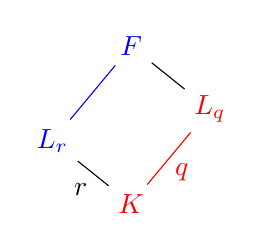
\begin{tikzpicture}

            \node [red] (Q1) at (0,0) {$K$};
            \node [red] (Q2) at (1,1.2) {$L_q$};
            \node [blue] (Q3) at (0,2) {$F$};
            \node [blue] (Q4) at (-1,0.8) {$L_r$};
        
            \draw [red] (Q1)--(Q2) node [pos=0.8, below,inner sep=0.25cm] {$q$};
            \draw (Q1)--(Q4) node [pos=0.9, below,inner sep=0.25cm] {$r$};
            \draw [blue] (Q3)--(Q4);
            \draw (Q2)--(Q3);
        
        \end{tikzpicture}
        \caption[short]{Subfields of a $C_{pq}$-extension}
    \end{figure}

    Again, the result follows immediately from the table and \eqref{eqn_local_contr}.
    
\end{proof}

We are finally ready to prove the main result of this section, from which Theorem \ref{thm_consistent_cyclic} will follow. 

\begin{lemma}\label{lem_Cd_odd}
    Let $d$ be a composite, odd squarefree integer and let $F/K$ be a Galois extension of number fields such that $\Gal(F/K)=C_{d}$. Let $E/\QQ$ be an elliptic curve with semistable reduction at $2$ and $3$ and let $L_k$ be the intermediate fields such that $\Gal(F/L_k)=C_{d/k}$. If 
    $$\Theta_d=\sum_{k\mid d}\mu(k)C_k\in B(C_d),$$
    then $C(\Theta_d)\in\QQss$.
\end{lemma}

\begin{proof}
    Let $n$ be the number of distinct prime numbers dividing $d$, so that $d=p_1\ldots p_n$ for some distinct odd primes $p_i$. We prove this result by induction. The base case for $n=2$ is the content of Lemma \ref{lem_Cpq}. Assume that the result holds for squarefree cyclic Galois extensions with $n-1$ prime factors and consider the two sets of subgroups
    $$\mathcal{A}=\{C_k:p_n\mid k\}\quad\text{and}\quad\mathcal{B}=\{C_k:p_n\nmid k\},$$
    which are clearly a partition of subgroups of $C_d$. Furthermore, the fields $\{F^{C_k}:C_k\in\mathcal{A}\}$ are precisely the intermediate fields of $L_{d/p_n}/K$, while the fields $\{F^{C_k}:C_k\in\mathcal{B}\}$ are the intermediate fields of $F/L_{p_n}$.
    Let 
    $$\Theta_\mathcal{A}=\sum_{H\in\mathcal{A}}\mu(|H|/p_n)H\quad\text{and}\quad\Theta_\mathcal{B}=\sum_{H\in\mathcal{B}}\mu(|H|)H$$
    and we note that
    \begin{equation}\label{eqn_theta}
        \Theta_d=\sum_{k\mid d}\mu(k)C_k=\sum_{p_n\nmid k\mid d}\mu(|C_k|)C_k-\sum_{p_n\mid k\mid d}\mu(|C_k|/p_n)C_k=\Theta_\mathcal{B}-\Theta_\mathcal{A}.
    \end{equation}
    Since $\Gal(L_{d/p_n}/K)=\Gal(F/L_{p_n})=C_{d/p_n}$, it follows from the inductive hypothesis applied to $L_{d/p_n}/K$ and $F/L_{p_n}$ that $C(\Theta_\mathcal{A}),C(\Theta_\mathcal{B})\in\QQss$, and therefore
    $$C(\Theta_d)=\frac{C(\Theta_\mathcal{B})}{C(\Theta_\mathcal{A})}\in\QQss,$$ 
    as desired.
    \begin{figure}[!ht]
        \centering
        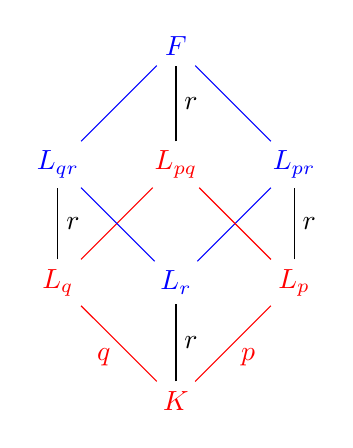
\begin{tikzpicture}

            \node [red] (Q1) at (0,0) {$K$};
            \node [red] (Q2) at (-1.5,1.5) {$L_q$};
            \node [blue] (Q3) at (0,1.5) {$L_r$};
            \node [red] (Q4) at (1.5,1.5) {$L_p$};
            \node [blue] (Q5) at (-1.5,3) {$L_{qr}$};
            \node [red] (Q6) at (0,3) {$L_{pq}$};
            \node [blue] (Q7) at (1.5,3) {$L_{pr}$};
            \node [blue] (Q8) at (0,4.5) {$F$};

            \draw [red] (Q1)--(Q2) node [pos=0.7, below,inner sep=0.25cm] {$q$};
            \draw [red] (Q1)--(Q4) node [pos=0.7, below,inner sep=0.25cm] {$p$};
            \draw (Q1)--(Q3) node [pos=0.5, right,inner sep=0.1cm] {$r$};
            \draw (Q2)--(Q5) node [pos=0.5, right,inner sep=0.1cm] {$r$};
            \draw (Q2)--(Q6) [red];
            \draw (Q3)--(Q5) [blue];
            \draw (Q3)--(Q7) [blue];
            \draw (Q4)--(Q6) [red];
            \draw (Q4)--(Q7) node [pos=0.5, right,inner sep=0.1cm] {$r$};
            \draw (Q5)--(Q8) [blue];
            \draw (Q6)--(Q8) node [pos=0.5, right,inner sep=0.1cm] {$r$};
            \draw (Q7)--(Q8) [blue];
        
        \end{tikzpicture}
        \caption[short]{Partition of $n=3$ into $n=2$. Red fields are in $\mathcal{A}$ while blue fields are in $\mathcal{B}$.}
    \end{figure}
\end{proof}

The proof of Theorem \ref{thm_consistent_cyclic} for odd $d$ is now straightforward.

\begin{proof}[Proof of Theorem \ref{thm_consistent_cyclic} for odd $d$]
    The proof is divided into two cases depending on whether $d$ is the power of a prime or not. Suppose first that $d$ is not, so that $\rad(d)$ is a squarefree \textbf{composite} number. Then $\Theta_d=\sum_{k\mid d}\mu(k)C_k\in B(C_d)$ is the $\psi_d$-relation of a faithful character of $C_d$. The subgroups appearing on $\Theta_d$ are the subgroups of $C_{\rad(d)}$ and therefore by Lemma \ref{lem_Cd_odd} applied to the $C_{\rad(d)}$ extension $F/F^{C_{\rad(d)}}$, it follows that 
    $$C(\Theta_d)\in\QQss,$$ and therefore it is the norm of an element for any quadratic extension of $\QQ$. 

    If $d=q^n$ for some odd prime $q$ and $n\geq1$, then Lemma \ref{lem_relation} shows that $\Theta_d=C_1-C_q$ is the $\psi_d$-relation of a faithful character of $C_d$. Lemma \ref{lem_Cp} applied to the $C_q$ extension $F/F^{C_q}$ proves that 
    $$C(\Theta_d)=\frac{C(C_1)}{C(C_q)}\in N_{\QQ(\sqrt{q^*})/\QQ}(\QQ(\sqrt{q^*})^{\times}).$$ 
    By Lemma \ref{lem_subfields} this is the only quadratic subfield of $\QQ(\zeta_{q^n})$, so the result follows.
\end{proof}
